\section{Deep Parameter Optimisation}

Figure \ref{system} shows the work flow of the deep parameter optimisation. The approach takes source code of a program under tuning, a set of test data and a set of non-functional properties of interests as inputs. 


It first applys mutation analysis to the program to generate a set of slight modified program. Each mutant is then executed with the set of test data.  All non-functional properties interestings are recording during the execution. All mutants are rank and 

Finnally it compbine and shadow and deep paramerter together and applys NSGAII to produce values for



Our approach takes three steps. Firstly we apply Mutation Operators to generate variants of the original \emph{dlmalloc} in order to understand which pieces of the source code could be more influential to the performance. Secondly we analyze the sensitivity of each mutated piece by evaluating the variants on a given set of applications and testsuites. After locating the most interesting and influential part of the code, we expose them to users so that they could be modified from the outside as needed. 

Thirdly, we apply SBSE approach to find the optimal values for both the existing and exposed parameters for each of the given applications.

\begin{figure}[htbp]
\centering
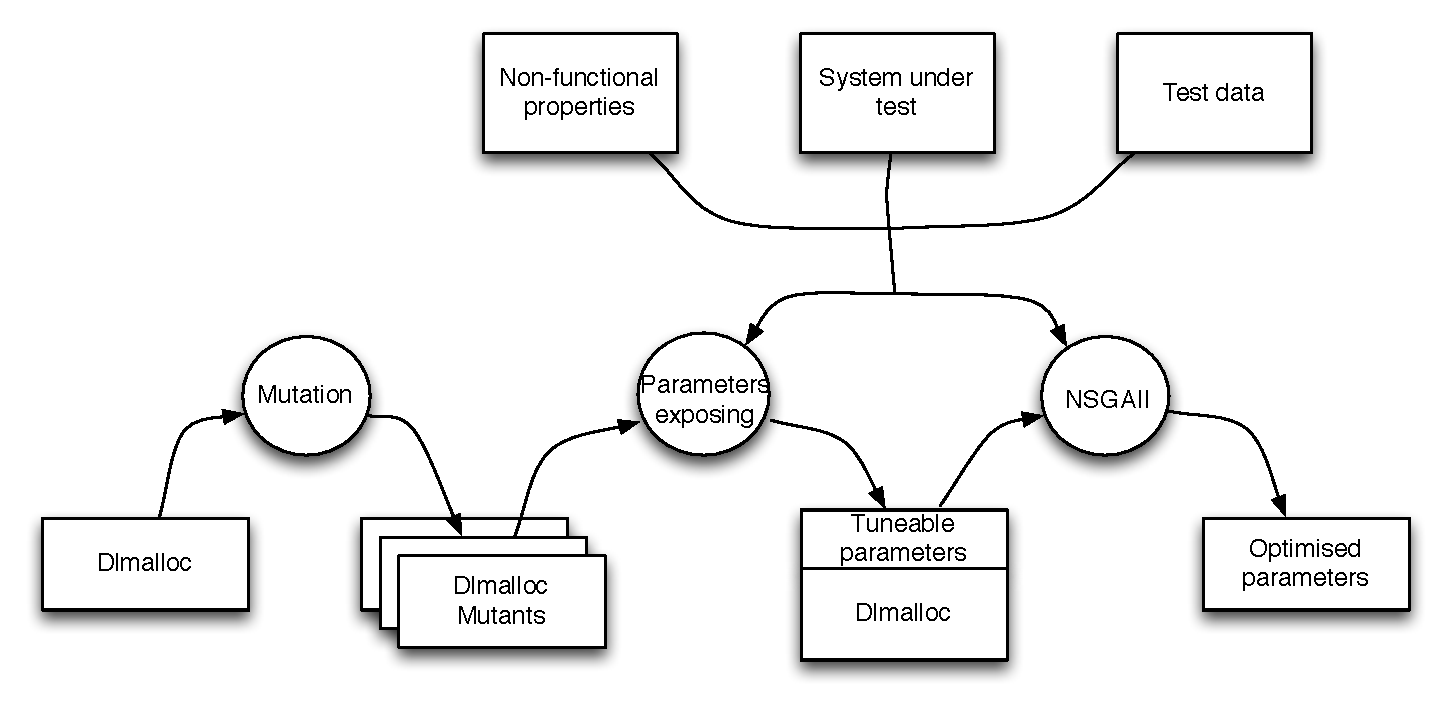
\includegraphics[width=3.2in]{pics/system}
\caption{Deep parameter optimisation workflow}\label{system}
\end{figure}


\subsection{Discovering locations for deep parameters}

The first step is to identify potential locations at which we could expose deep parameters. 
In our approach, we represents the input program as an abstract syntax tree and a potential location $L$ is an expression node of the AST. 
We want to find locations $L_D$ such that when we change the value of the expression at $L_D$, some non-functional properties of the program are improved while the program remains the same functional behaviour. 
We use software testing to valid the functional behaviour of the program. 

We use mutation analysis to automatically search for locations $L_D$. Mutant analysis deliberately makes simple syntactic changes to the input program, to create a set of various version programs called mutants, each contains a different syntactic change. A transformation rule that generates a mutant from the input program is know as a mutation operator. By carefully choosing mutation operators, we can use mutants to simulate the effect of making changes all potential location $L$ . Table \ref{tab:cmop} shows the operator we used to generate mutants, covering locations of a constants, relational, logical and arithmetic expressions. 
To assess the quality of a mutant, we test each mutant against the input test set and record the values of the non-functional properties. 

\begin{table} [htbp]
\caption{Selected mutation operators}
\label{tab:cmop} 
\begin{center}
\begin{tabular}{ | c | l |}
  \hline
  Mutation Operators & Description \\ 
\hline
  CRCR & Required constant replacement \\
  OAAN & Arithmetic operator mutation \\
  OAAA & Arithmetic assignment mutation \\
  OCNG & Logical context negation \\
  OIDO & Increment/decrement mutation  \\
  OLLN & Logical operator mutation  \\ 
  OLNG & Logical negation \\
  ORRN & Relational operator mutation \\
  OBBA & Bitwise assignment mutation \\
  OBBN & Bitwise operator mutation \\
\hline
\end{tabular} 
\end{center} 
\end{table} 

After the mutants are tested, we first filter out those mutants which fail to hold the functionality, thus only the equivalent mutants are preserved. Practically, we cannot expose parameters from all potential locations, which drives us to search for the locations which could have the greatest impact on the non-functional properties. We achieve this by looking at each mutant's non-functional properties, based on which we then sort them with respect to a non-dominated sorting approach used in NSGA II\cite{}. That is, assigning the Pareto Level and Crowd Distance to each mutant, where Pareto Level $n$ means a mutant will be on the Pareto Front after all the mutants with Pareto Level less than $n$ are removed, while Crowd Distance indicates how close a mutant is to its neighbors on the same Pareto Level. Then a mutant is better than another in terms of non-dominated sorting if its Pareto Level is smaller or their Pareto Level is the same but the former is less crowded (bigger Crowd Distance) than the latter. After sorting all the mutants in terms of their non-functional properties, we apply a greedy algorithm to pick $k$ locations that could best influence the non-functional properties of the original but don't cover each other, the algorithm is described in Figure ?.

%\begin{algorithm}
%	Sort the mutants in terms of their non-functional properties and non-dominated sorting: m1, m2, ..., mn\;
%	$LS=\emptyset, i=1$\;
%	While{$|LS|<k$}{
%		$LS=LS \cup \{L\}, \text{if} L \text{involves} L_mi \&\& \forall L' \in LS, L' \text{doesn't cover} L$
%		$i=i+1$
%	}
%	\caption{Greedy algorithm to choose locations to expose}
%\end{algorithm}

In the algorithm, $k$ is the desired number of Deep Parameters one wants to expose. 

%
%
%where if we make an modification, coudhave a great affect on the  escribe how we define a Deep Parameter and how we choose and expose these Deep Parameters.
%
%We define a Deep Parameter by starting from defining a location from which a Deep Parameter is exposed.
%
% A location $L$ is an expression that meets:
%\begin{equation}
%L: \mbox{CONSTANT} | \mbox{IDENTIFIER} | L\ binary-op\ L | unary-op\ L
%\end{equation}
%
%where the $binary-op$ can be a relational operator (>, <, >=, <=, ==, !=), a logical operator (\&\&, ||, !) or an arithmetic operator (+, -, *, /, \%). 
%
%So a location can be a constant, a variable or an expression derived from other location(s) with an operator. 
%
%When a location is composed of other location(s) and an operator $op$ and the $op$ is a relational operator or a logical operator, we call it a logical location, otherwise it is an arithmetic location. 
%
%
%Apparently, exposing parameters from all possible locations from a program will give users the maximum capacity to control the behaviour of the program. However, since we want to optimize these Deep Parameters as well as Shallow Parameters on a given test suite, it is impractical to expose and optimize all of possible Deep Parameters. So we firstly need to determine which locations to expose.

%In theory, we can expose parameter from each legible location and optimize the parameter on a given test suite, to understand how much better performance of the program under optimise we can achieve by tuning this parameter. Formally, $E_{LS}(L)$ is the best performance of a program after exposing and optimizing parameter $v$ from location $L$:
%\begin{equation}
%E_{LS}(L)=\max_{a} E_T(P(L)|_{v=a}),
%\end{equation}
%where $E_T()$ is a function which evaluate a program's performance on a given test suite $T$. However, it may needs infinitely large number of evaluations due to the infinite possible values of $a$. Instead, we propose a Mutation-based approach to analyse how likely we could achieve better performance by exposing one parameter than another.
%
%\subsection{Mutation analyse **}
%(** old)
%In order to obtain the sensitivity information, one simple way is to delete each statement at a time to see how important this statement is to the performance of \emph{dlmalloc}. However, when the statement deleted is consist of a very complicated expression, which variable or operator is more important than others remains unknown. 
%
%A more advanced way to obtain the sensitivity information is via Mutation Operators. Mutation Operators are used in Mutation Testing, which automatically inserts some faults to a target program via Mutation Operators to generate mutants of this program and try to detect those faults using a test suite to see whether the test suite is good enough to reveal program faults. 
%
%In this work, we just use these Mutation Operators to slightly alter \emph{dlmalloc}, in order to understand which piece of source code influences the memory consumption most. We apply both the statement deletion way and Mutation Operator way in the sensitivity analysis and compare their effectiveness, which is reported later. In either way, there are many variants of original \emph{dlmalloc} generated, all of them only differ from the original in at most one statement. We then evaluate and record the performance of these variants on the subject applications and corresponding test suites. This helps us understand the most influential pieces of code in the original \emph{dlmalloc}.
%
%(** fannew)
%Mutation Operators are originally used in Mutation Testing to automatically insert artificial faults to a program under test, generating different versions, or mutants, of the original program. These mutants are later test under a given test suite trying to discover those artificial faults as a means of revealing how good the test suite is for detecting real faults. Here we only use Mutation Operators to generate mutants that slightly differ from the original program. According to the Mutation Operators we used, the mutated location $L_m$ can be a constant, a relational operator, a logical operator, an arithmetic operator or a predicate. Then we say a location $L$ involves a mutated location $L_m$ if $L_m$ is a substring of $L$. By this definition, we can approximate $E_{LS}(L)$ by evaluating the best performance of the mutants whose mutated location $L_m$ is involved by $L$. 
%
%Notice that from the same statement, there could be multiple locations by our definition. For example, from the statement $a=b+c$, there are three locations: $L_1:b$, $L_2:c$, $L_3:b+c$. Apparently, exposing parameters from each of them will result in semantically the same program. So if we find exposing parameter from location $L_3$, there is no need to expose more parameters from the other two locations. We say a location $L_a$ covers location $L_b$ if $L_b$ is a substring of $L_a$. For example, locations $L_3$ covers both location $L_1$ and $L_2$ in the previous example. 
%
%(**describe the greedy algorithm we used to choose $k$ location to expose)
%
%(**describe how we apply our approach on the dlmalloc case study, including separately finding best locations to expose with respect to each subject application)
%

\subsection{Exposing deep parameters}
The second step is to expose deep parameters which allow users to modify the values of the expression at selected locations. Based on the type of mutation, we first classify the selected mutants into two sets. $Set\ 1$ includes contains mutants generated from the CRCR, OAAN, OAAA and OIDO operators, which simulate locations with non-logical expression. $Set\ 2$ constrains mutants generated from the OCNG, OLLN, OLNG and ORRN operators, which simulate locations with non-logical. 
Give an location $L$, $E_L$ is the expression at the location $L$, we use the following transformation rules to rewrite the $E_L$ with a new parameter $v$.

\begin{equation}
 E_L \rightarrow \left\{
  \begin{array}{l l}
    (E_L + v) & \quad \text{if $L$ $\in$ Set 1}\\
    (E_L) \ xor \ v & \quad \text{if $L$ $\in$ Set 2}
    \end{array} \right.
\end{equation}

We use addition to affect the value of non-logical expression and exclusive or to affect the logical ones.
Finally we expose $v$ as a `public' parameter so that users can assign value to $v$ through parameter passing or APIs.

\subsection{MultiObjective Paramter optimisation}
\label{sec_nsgaii}
In this work, we apply NSGA II\cite{996017}, a multi-objective Genetic Algorithm, on the searching of the optimal values for those \emph{dlmalloc} parameters list above.
% data representation
Since these parameters can be easily interpreted as integers, we use linear representation to store each candidate, in which each gene is an integer number representing one of the parameters. For mutation, we use different operators according to each gene's legitimate range, while two-point crossover is applied.
% fittness evaluation

Since we need to re-compile \emph{dlmalloc} every time we change the parameters, in order to minimize compilation cost, we only compile \emph{dlmalloc} to a shared object and each application is compiled and linked to that shared object at the beginning of each experiment. In each generation, after new candidates are generated through mutation and crossover operators, each candidate is re-compiled and run with a given subject application. When the performance of the application with each candidate version of \emph{dlmalloc} is collected, an NSGA II style selection is applied to obtain the next generation.
% how to measure time
% how to measure memory

Currently we focus on two non-functional properties: time and memory consumption. \emph{Glibc}'s \emph{wait4} function is used to calculate the cpu time consumed by the application (sum of user time and system time), while we compute the high-water mark of the memory consumption by instrumentation of \emph{dlmalloc}. In this way the memory measured is virtual memory, because the physical pages allocated to an application is not always deterministic but depends on the work load and the system so that measuring the physical memory usage could be hard and misleading.

